\documentclass{article}
\usepackage{pgfplots}
\begin{document}

\noindent Justin Stanley \\
Design and Analysis of Algorithms \\
October 15, 2015 \\
Extra-Credit Assignment 1 \\

\hrulefill

The task presented was to develop a program implementing the selection and bubble sort algorithms,
and to analyze the times taken for different input sizes contrasted with the algorithm's computational complexity $\mathcal{O}(f(n))$.

I implemented the algorithms in two different languages and also did some further testing to illustrate the relationship between input size and computing time.
The first data provided will be the results for the selection sort

\begin{center}
	\textit{Time (milliseconds) to sort elements, assignment-given tests}
	\begin{tabular}{l | r | r}
		Implementation & $n$=5000 & $n$=50000 \\ \hline
		Selection [ISO C99] & 25.211 & 1854.049 \\ \hline
		Selection [Python 3.5] & 1299.779 & 154338.610 \\ \hline
		Bubble [ISO C99] & 65.803 & 5637.274 \\ \hline
		Bubble [Python 3.5] & 5906.187 & 736724.950 \\
	\end{tabular}
\end{center}

We know from previous analysis of the selection sort and the bubble sort that both algorithms belong to the complexity class $\mathcal{O}(n^2)$. To predict the times for $n$=50000 given only the time for $n$=5000, we would have to take that into account. We know that both algorithms operate on an order of $n^2$, with some deviation due to startup time and other time spent not related to the algorithm. To find the time it takes to perform one basic operation $k$, we divide the time $t$ taken by the algorithm to compute by the number of elementary operations $n^2$.

Given the time to compute a basic operation $k$, we can compute the estimated amount of time for an input size $n$ by calculating $kn^2$. The calculations can be shown for the selection sort [Python] with $n=5000$ vs $n=50000$:

\begin{center}
	$k = \frac{5000^2}{1299.779 ms} = 5.1991 * 10^{- 5}$ ms \\
	$t = k*50000^2 = 129977.9$ ms (\textit{actual result 154338.6 ms})
\end{center}

This prediction has only 15\% error (24360.7 ms) and came reasonably close to the actual result. Sources of error include floating-point precision (the time in milliseconds for an elementary operation is very small), as well as confounding variables in the execution environment. Linux is a multitasking kernel and not all programs will always receive sufficient CPU time for consistent results.

The following pages will contain a more in-depth analysis of the performance of the two languages and the performance of the two algorithms.

\newpage

The extended analysis tested three ranges of values for both of the algorithms. The language names are abbreviated in the table as to preserve room.

\begin{center}
	\textit{Time (milliseconds) to sort elements, small-scale tests}
	\begin{tabular}{l | r | r | r | r | r}
		& $n=128$ & $n=256$ & $n=384$ & $n=512$ & $n=640$ \\ \hline
		Selection [C] & 0.055 & 0.211 & 0.469 & 0.830 & 1.336 \\ \hline
		Selection [Py] & 0.752 & 2.645 & 7.958 & 15.038 & 21.902 \\ \hline
		Bubble [C] & 0.128 & 0.572 & 1.328 & 2.300 & 3.805 \\ \hline
		Bubble [Py] & 2.805 & 12.098 & 32.168 & 55.175 & 96.536 \\
	\end{tabular}
\end{center}

\begin{center}
	\textit{Time (milliseconds) to sort elements, medium-scale tests}
	\begin{tabular}{l | r | r | r | r | r}
		& $n=2048$ & $n=4096$ & $n=6144$ & $n=8192$ & $n=10240$ \\ \hline
		Selection [C] & 12.252 & 24.137 & 39.507 & 57.308 & 85.884 \\ \hline
		Selection [Py] & 236.447 & 953.649 & 1943.829 & 3532.748 & 5760.187 \\ \hline
		Bubble [C] & 15.804 & 44.319 & 94.440 & 159.352 & 248.895 \\ \hline
		Bubble [Py] & 1012.824 & 3993.341 & 9254.053 & 15841.523 & 25239.121 \\
	\end{tabular}
\end{center}

\begin{center}
	\textit{Time (milliseonds) to sort elements, large-scale tests}
	\begin{tabular}{l | r | r | r | r | r}
		& $n=16384$ & $n=32768$ & $n=49152$ & $n=65536$ \\ \hline
		Selection [C] & 205.684 & 814.151 & 1792.096 & 3181.213 \\ \hline
		Selection [Py] & 13976.302 & 58543.965 & 131223.770 & 240732.600 \\ \hline
		Bubble [C] & 618.205 & 2426.378 & 5414.361 & 9614.802 \\ \hline
		Bubble [Py] & 62854.785 & 264360.650 & 594066.920 & 1060772.400 \\
	\end{tabular}
\end{center}

The last test of the large-scale group was omitted as the Python implementation was predicted to take an unreasonable amount of time to compute the solution. The analysis and contrast between the two implementations is surprising, especially considering the large-scale bubble sort. The Python implementation seems to take significantly longer to compute the solutions, in this case by a factor greater than 1000. The graph of the respective tests certainly demonstrates a difference in both absolute performance and relative growth.

\begin{center}
	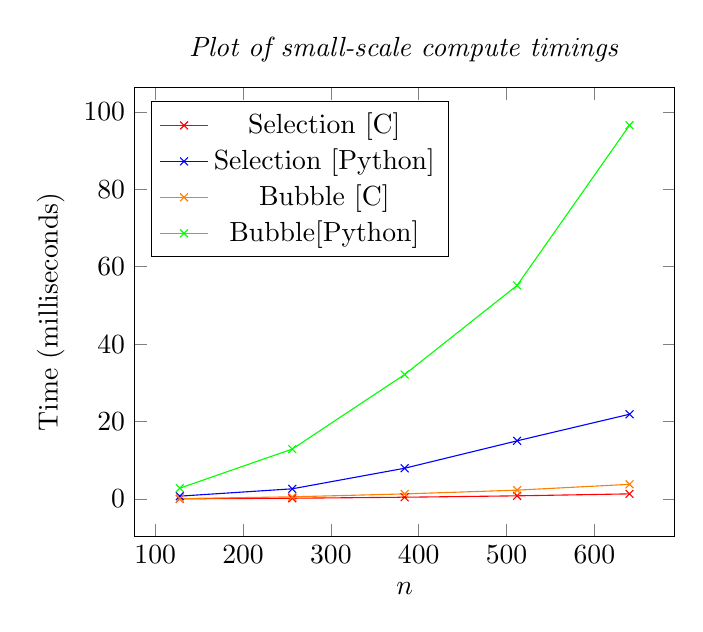
\begin{tikzpicture}
		\begin{axis}[xlabel=$n$,ylabel={Time (milliseconds)},title={\textit{Plot of small-scale compute timings}},legend pos=north west]
			\addplot[color=red,mark=x] coordinates {
				(128, 0.055)
				(256, 0.211)
				(384, 0.469)
				(512, 0.830)
				(640, 1.336)
			};
			\addplot[color=blue,mark=x] coordinates {
				(128, 0.752)
				(256, 2.645)
				(384, 7.958)
				(512, 15.038)
				(640, 21.902)
			};
			\addplot[color=orange,mark=x] coordinates {
				(128, 0.123)
				(256, 0.572)
				(384, 1.328)
				(512, 2.300)
				(640, 3.805)
			};
			\addplot[color=green,mark=x] coordinates {
				(128, 2.805)
				(256, 12.908)
				(384, 32.168)
				(512, 55.175)
				(640, 96.536)
			};
			\legend{Selection [C], Selection [Python], Bubble [C], Bubble[Python]}
		\end{axis}
	\end{tikzpicture}
\end{center}

The small-scale graph definitely shows a major difference in performance vs input size, with Python and C performing similarly for very small inputs but Python growing in complexity much faster than C. Around 512, there is already a major difference in performance between Python and C. This difference in growth can be seen in the later graphs as well, with a much higher magnitude. Both bubble sort are significantly slower than their selection sort counterparts.

\begin{center}
	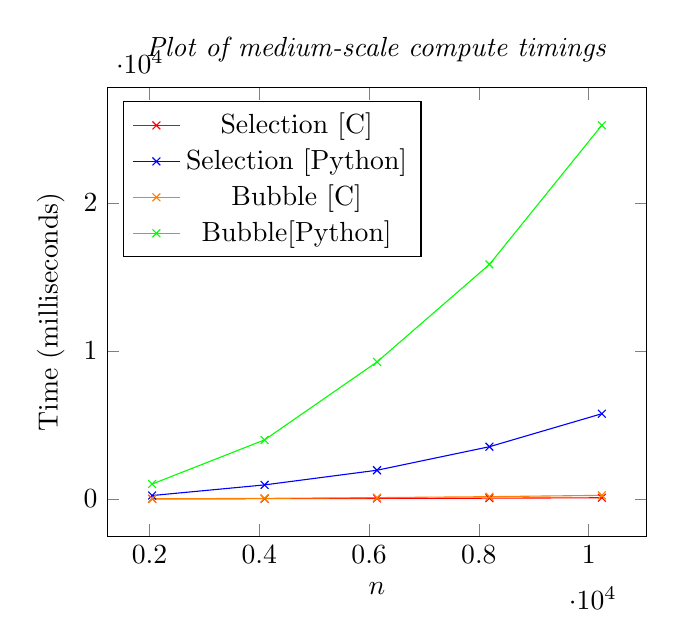
\begin{tikzpicture}
		\begin{axis}[xlabel=$n$,ylabel={Time (milliseconds)},title={\textit{Plot of medium-scale compute timings}},legend pos=north west]
			\addplot[color=red,mark=x] coordinates {
				(2048, 13.252)
				(4096, 24.137)
				(6144, 39.507)
				(8192, 57.308)
				(10240, 85.884)
			};
			\addplot[color=blue,mark=x] coordinates {
				(2048, 236.447)
				(4096, 953.649)
				(6144, 1943.829)
				(8192, 3532.748)
				(10240, 5760.187)
			};
			\addplot[color=orange,mark=x] coordinates {
				(2048, 15.804)
				(4096, 44.319)
				(6144, 94.440)
				(8192, 159.352)
				(10240, 248.895)
			};
			\addplot[color=green,mark=x] coordinates {
				(2048, 1012.824)
				(4096, 3993.341)
				(6144, 9254.053)
				(8192, 15841.523)
				(10240, 25239.121)
			};
			\legend{Selection [C], Selection [Python], Bubble [C], Bubble[Python]}
		\end{axis}
	\end{tikzpicture}
\end{center}

This graph appears to resemble the small-scale plot remarkably. The plot of the C timings appears to not be increasing as much. The Python timings continue to increase greatly, while the C performance seems to be very close to 0 in comparison. The difference in performance between the bubble sort and the selection sort seems to be much greater in Python than in C. The Python bubble sort algorithm is quickly identified as the least effective algorithm amongst the other for large input sizes.

\begin{center}
	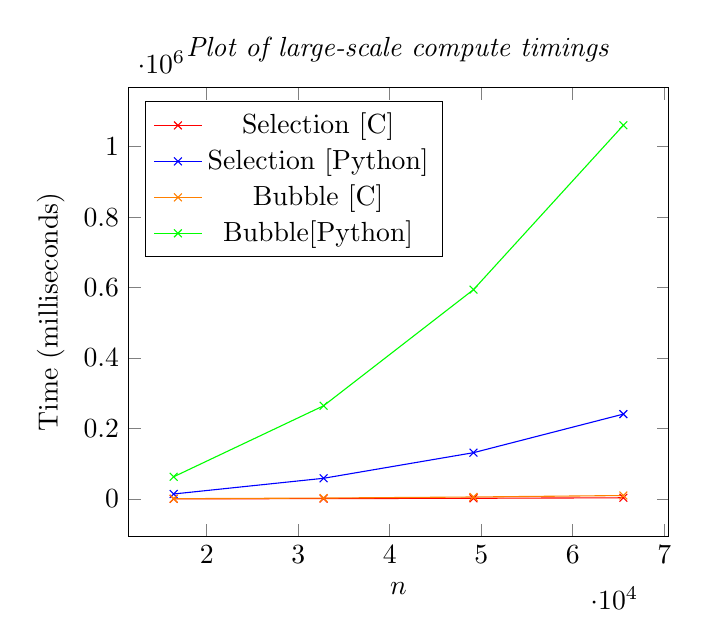
\begin{tikzpicture}
		\begin{axis}[xlabel=$n$,ylabel={Time (milliseconds)},title={\textit{Plot of large-scale compute timings}},legend pos=north west]
			\addplot[color=red,mark=x] coordinates {
				(16384, 205.684)
				(32768, 814.151)
				(49152, 1792.906)
				(65536, 3181.213)
			};
			\addplot[color=blue,mark=x] coordinates {
				(16384, 13976.302)
				(32768, 58543.965)
				(49152, 131223.77)
				(65536, 240732.60)
			};
			\addplot[color=orange,mark=x] coordinates {
				(16384, 618.205)
				(32768, 2426.378)
				(49152, 5414.361)
				(65536, 9614.802)
			};
			\addplot[color=green,mark=x] coordinates {
				(16384, 62854.785)
				(32768, 264360.65)
				(49152, 594066.92)
				(65536, 1060772.4)
			};
			\legend{Selection [C], Selection [Python], Bubble [C], Bubble[Python]}
		\end{axis}
	\end{tikzpicture}
\end{center}

As expected, the graph of the large-scale compute times resembles the other graphs as well. The Python implementation appears to be consistent with the $n^2$ growth rate compared to C. Interestingly, the information gathered on the C implementation timings actually \textit{does} resemble $n^2$ growth. It seems that the Python implementation distorts the scale of the graph significantly enough to hide the fact that the C implementation is indeed growing at an $n^2$ rate. The scale of the graph is also misleading as to the difference in performance between the C selection sort and the C bubble sort, which turns out to be substantial.

The algorithms examined in this assignment and their respective implementations have several differences. Both the bubble sort and the selection sort algorithms belong to $\mathcal{O}(n^2)$, but bubble sort appears to consistently perform worse than the selection sort for both implementations. This difference can be explained with the fact that $\mathcal{O}$ does not describe immediate complexity differences but rather complexity growth as input size increases to large values. The bubble sort algorithm has the same growth over time as the selection sort algorithm, but the selection sort tends to generally be much faster for small inputs. This could be due to the nature of the bubble sort algorithm, which requires significantly more swaps and temporary stack variables than the selection sort. The bubble sort also must create and destroy temporary variables significantly more than the selection sort does. This explains the difference in performance between the selection sort and the bubble sort algorithms.

The two languages also appear to have a clear performance difference. The Python implementations used appear to consistently perform worse than the C implementations. This has a much simpler explanation: C is compiled to native code and does not require a hypervisor to execute instructions. Python runs under a virtual environment and must make the equivalent of several operations in C to perform basic operations. Python is also interpreted, not compiled in this instance. This explains the large gap in performance as well as the larger time growth for input size.

\end{document}
